\section{Detailed Experiments}

\subsection{Stack (Array version)}

\subsubsection{Push operators}

\begin{figure}[H]
    \centering
    \subfloat[\centering Normal case]{{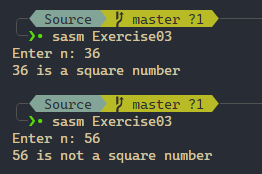
\includegraphics[width=5cm]{img/img3.png} }}%
    \qquad
    \subfloat[\centering Full case]{{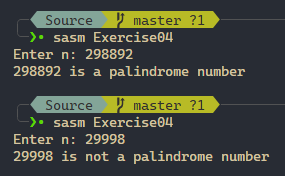
\includegraphics[width=5cm]{img/img4.png} }}%
    \caption{Push element in Stack by Array (size=5)}%
    \label{fig:stackArrayPush}%
\end{figure}
\subsubsection{Pop operators}

\begin{figure}[H]
    \centering
    \subfloat[\centering Normal case]{{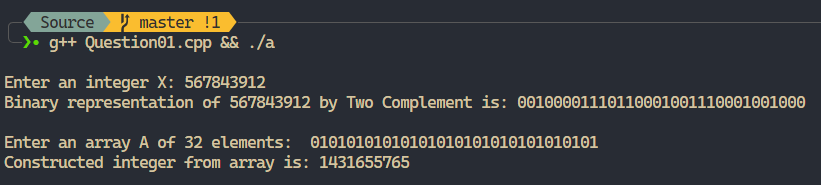
\includegraphics[width=5cm]{img/img1.png} }}%
    \qquad
    \subfloat[\centering Empty case]{{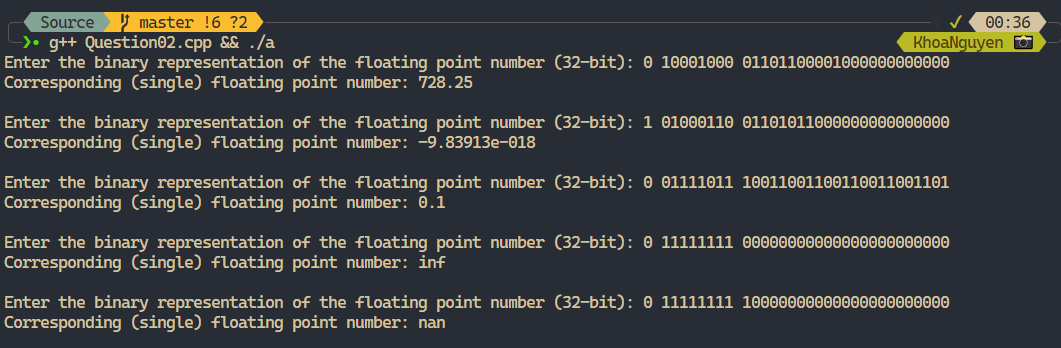
\includegraphics[width=5cm]{img/img2.png} }}%
    \caption{Pop element in Stack by Array}%
    \label{fig:stackArrayPop}%
\end{figure}

\subsection{Stack (Linked List version)}

\subsubsection{Push operators}
Implement the Stack by singly linked list is created by dynamic allocation, does not require a fixed size when declaring. Therefore, we can add or remove elements easily without changing the original declaration and there is no maximum size when declared as an array.\\
Therefore, the size of the Stack will depend on the computer's RAM memory.\\

\begin{figure}[H]
    \centering
    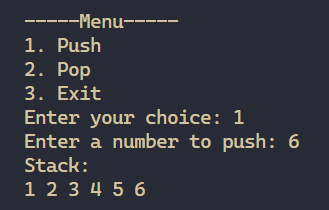
\includegraphics{img/img7.PNG}
    \caption{Push element in Stack by Linked List}
    \label{fig:stackLinkedListPush}
\end{figure}

\subsubsection{Pop operators}

\begin{figure}[H]
    \centering
    \subfloat[\centering Normal case]{{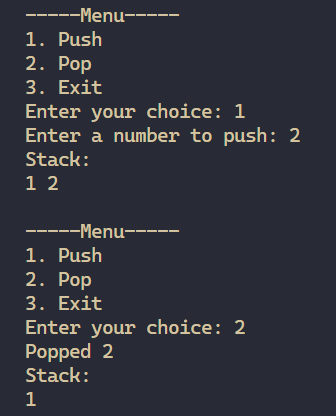
\includegraphics[width=5cm]{img/img5.png} }}%
    \qquad
    \subfloat[\centering Empty case]{{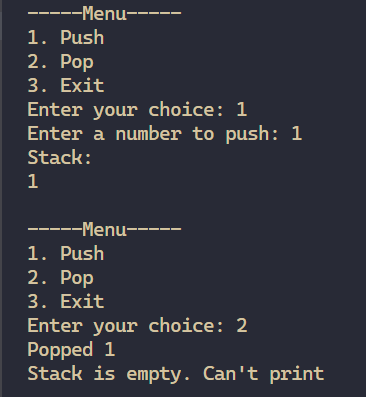
\includegraphics[width=5cm]{img/img6.png} }}%
    \caption{Pop element in Stack by Linked List}%
    \label{fig:stackLinkedListPop}%
\end{figure}

\subsection{Queue (Array version)}

\subsubsection{Enqueue operators}

\begin{figure}[H]
    \centering
    \subfloat[\centering Normal case]{{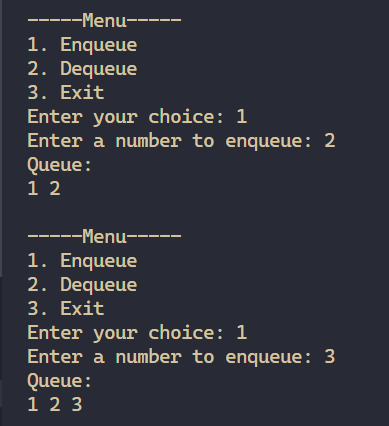
\includegraphics[width=5cm]{img/img9.PNG} }}%
    \qquad
    \subfloat[\centering Full case]{{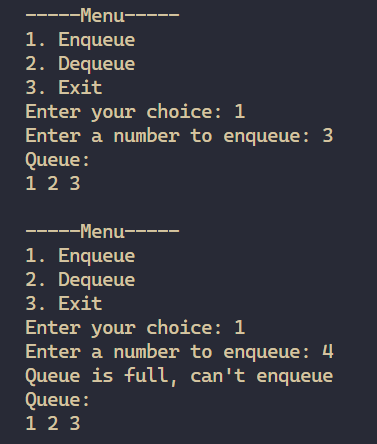
\includegraphics[width=5cm]{img/img10.png} }}%
    \caption{Enqueue element in Queue by Array}%
    \label{fig:queueArrayEnqueue}%
\end{figure}

\subsubsection{Dequeue operators}
\begin{figure}[H]
    \centering
    \subfloat[\centering Normal case]{{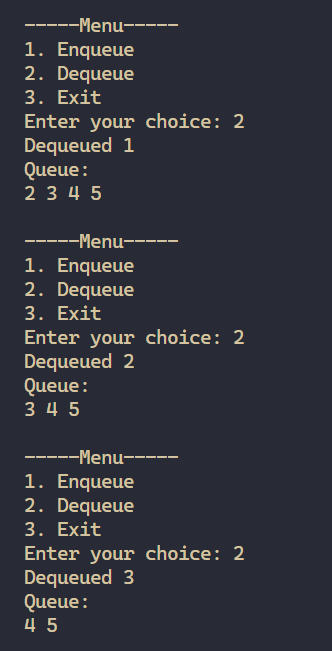
\includegraphics[width=5cm]{img/img11.PNG} }}%
    \qquad
    \subfloat[\centering Empty case]{{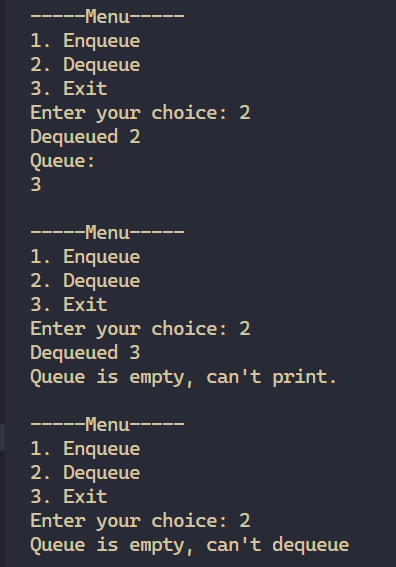
\includegraphics[width=5cm]{img/img12.png} }}%
    \caption{Dequeue element in Queue by Array}%
    \label{fig:queueArrayDequeue}%
\end{figure}


\subsection{Queue (Linked List version)}
\subsubsection{Enqueue operators}
Similar to Stack initialized with Linked List, Queue initialized with Linked List also does not have a maximum size. Therefore, the size of the Queue will depend on the computer's RAM.\\

\begin{figure}[H]
    \centering
    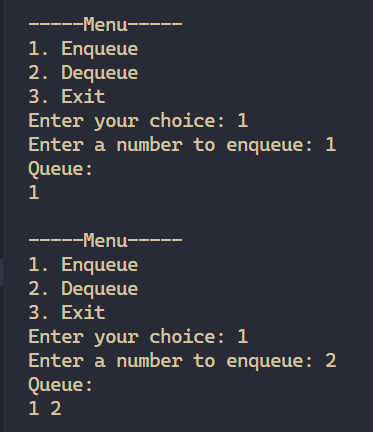
\includegraphics[width=6cm]{img/img13.PNG}
    \caption{Enqueue element in Queue by Linked List}
    \label{fig:QueueLinkedListEnqueue}
\end{figure}

\subsubsection{Dequeue operators}
\begin{figure}[H]
    \centering
    \subfloat[\centering Normal case]{{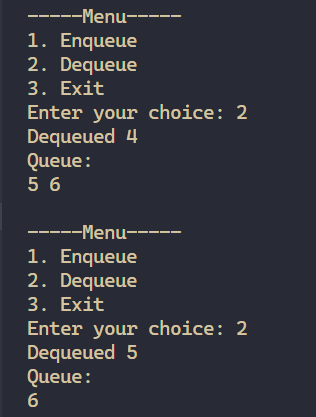
\includegraphics[width=5cm]{img/img14.PNG} }}%
    \qquad
    \subfloat[\centering Empty case]{{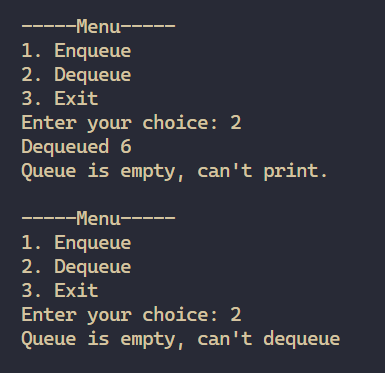
\includegraphics[width=5cm]{img/img15.PNG} }}%
    \caption{Dequeue element in Queue by Linked List}%
    \label{fig:queueLinkedListDequeue}%
\end{figure}
\newpage
\subsection{Recursion Version}
Recursive functions can be slower than loops due to overheads of function calls, more memory usage due to recursive calls added to the stack, and potential repetitive computations. Loops are generally more efficient, but recursion can offer simpler solutions for some problems.\\
I utilized the function from the Chrono library to measure and compare the running time of the algorithm. \cite{Measure_time_in_C++}

\subsubsection{Stack}
\subsubsection*{Array version}
\begin{figure}[H]
    \centering
    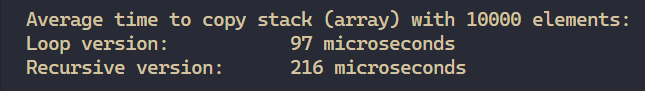
\includegraphics[width=13cm]{img/img16.PNG}
    \caption{Compare time loop and recursive version of Stack(Array)}
    \label{fig:StackArrayCompare}
\end{figure}
\begin{itemize}
    \item  Both implementations function copy Array have a time complexity of \textbf{O(n)} and the loop version is faster than recursive version.
\end{itemize}
The system will have a \textbf{Stack Overflow} if using an array with a recursive version with a large number of elements (above $10^{8}$ elements).

\subsubsection*{Linked List version}
\begin{figure}[H]
    \centering
    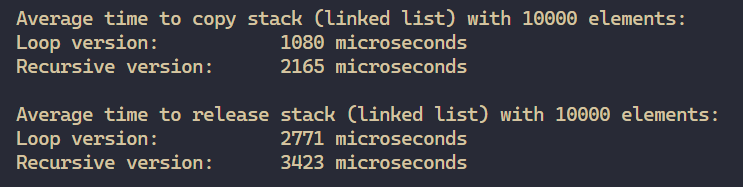
\includegraphics[width=13cm]{img/img17.PNG}
    \caption{Compare time loop and recursive version of Stack(Linked List)}
    \label{fig:StackLinkedListCompare}
\end{figure}
\begin{itemize}
    \item  Both implementations function copy and release Linked List have a time complexity of \textbf{O(n)} and the loop version is faster than recursive version.
\end{itemize}

\subsubsection{Queue}
\subsubsection*{Array version}
\begin{figure}[H]
    \centering
    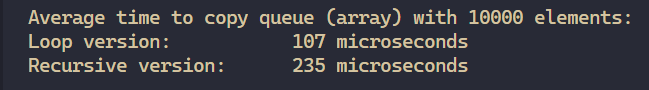
\includegraphics[width=13cm]{img/img18.PNG}
    \caption{Compare time loop and recursive version of Queue(Array)}
    \label{fig:QueueArrayCompare}
\end{figure}
\begin{itemize}
    \item  Both implementations function copy Array have a time complexity of \textbf{O(n)} and the loop version is faster than recursive version.
\end{itemize}
The system will have a \textbf{Stack Overflow} if using an array with a recursive version with a large number of elements (above $10^{8}$ elements).
\subsubsection*{Linked List version}
\begin{figure}[H]
    \centering
    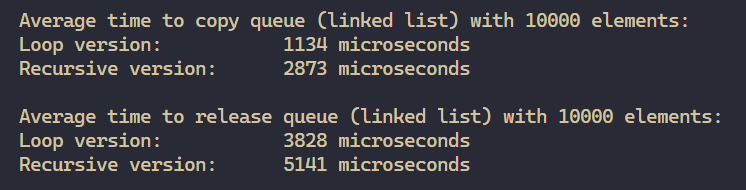
\includegraphics[width=13cm]{img/img19.PNG}
    \caption{Compare time loop and recursive version of Queue(Linked List)}
    \label{fig:QueueLinkedListCompare}
\end{figure}

\begin{itemize}
    \item  Both implementations function copy and release Linked List have a time complexity of \textbf{O(n)} and the loop version is faster than recursive version.
\end{itemize}



